\section{The Bipartisan Paxos Protocols}
The BPaxos protocols implement state machine replication. Informally, a set of
clients propose commands to a set of replicas, and the replicas execute the
commands in the same order (modulo reordering of non-conflicting commands). In
this section, we formalize state machine replication by way of generalized
consensus on conflict graphs. We then overview the common structure that
underlies all of the BPaxos protocols.

\subsection{Problem Description}
{\begin{figure}[h]
  \centering
  \tikzstyle{vertex}=[]
  \tikzstyle{arrow}=[thick, -latex]
  \tikzstyle{hidden}=[gray!50]

  \begin{subfigure}[b]{1.4in}
    \centering
    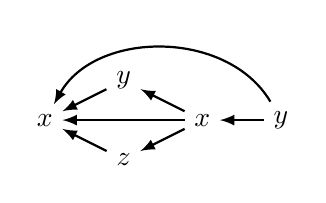
\begin{tikzpicture}
      \node[vertex] (x1) at (0, 0) {$x$};
      \node[vertex] (y1) at (1, 0.5) {$y$};
      \node[vertex] (y2) at (1, -0.5) {$z$};
      \node[vertex] (x2) at (2, 0) {$x$};
      \node[vertex] (z) at (3, 0) {$y$};

      \draw[arrow] (y1) to (x1);
      \draw[arrow] (y2) to (x1);
      \draw[arrow] (x2) to (y1);
      \draw[arrow] (x2) to (y2);
      \draw[arrow] (x2) to (x1);
      \draw[arrow, bend right=60] (z) to (x1);
      \draw[arrow] (z) to (x2);
    \end{tikzpicture}
    \caption{A conflict graph $C$}\figlabel{ExampleConflictGraph}
  \end{subfigure}%
  \hspace{1in}
  %
  \begin{subfigure}[b]{1.4in}
    \centering
    \begin{tikzpicture}
      \node[vertex] (x1) at (0, 0) {$x$};
      \node[vertex] (y1) at (1, 0.5) {$y$};
      \node[vertex] (y2) at (1, -0.5) {$z$};
      \node[vertex] (x2) at (2, 0) {$x$};
      \node[vertex, hidden] (z) at (3, 0) {$y$};

      \draw[arrow] (y1) to (x1);
      \draw[arrow] (y2) to (x1);
      \draw[arrow] (x2) to (y1);
      \draw[arrow] (x2) to (y2);
      \draw[arrow] (x2) to (x1);
      \draw[arrow, bend right=60, hidden] (z) to (x1);
      \draw[arrow, hidden] (z) to (x2);
    \end{tikzpicture}
    \caption{A suffix of $C$}\figlabel{ExampleSuffix}
  \end{subfigure}

  \caption{}
\end{figure}
}

Consider a set $\Cmd$ of commands and a binary reflexive relation $\conflict$
over $\Cmd$. We say two commands $x$ and $y$ \defword{conflict} if $(x, y) \in
\conflict$, and we say they are \defword{independent} otherwise. A
\defword{conflict graph} (over $\conflict$) is a directed acyclic graph such
that every vertex is labelled with a command and an edge is drawn between two
vertices if and only if they are labelled with commands that conflict (with
respect to $\conflict$)~\cite{mazurkiewicz1995introduction}.

We associate every conflict graph with the set of command strings that can be
obtained by a reverse topological sort of the conflict graph. For example,
consider the conflict graph over $\conflict$ shown in
\figref{ExampleConflictGraph} where
  $\conflict = \set{(x, x), (x, y), (y, x), (x, z), (z, x)}$.
The conflict graph can be reverse topological sorted in two ways, yielding the
two command strings $xyzxy$ and $xzyxy$. Moreover, notice that these two
command strings can be obtained from one another by interchanging their second
and third commands. This is true in general. Any two command strings of a
conflict graph can be obtained from the other by repeatedly interchanging
adjacent independent commands. These sets of command strings are known as
Mazurkiewicz traces~\cite{mazurkiewicz1985semantics,
mazurkiewicz1995introduction} and formalize the orders in which replicated
state machines can execute commands while remaining in sync.

Let $G = (V, E, \varphi)$ be a conflict graph where $V$ is the set of vertices,
$E \subseteq V \times V$ is the set of edges, and $\varphi: V \to \Cmd$ is the
labelling function that assigns a command to every vertex. We say $G' = (V',
E', \varphi|_{V'})$ is a \defword{suffix} of $G$ if $G'$ is a subgraph of $G$
such that for every edge $(v_1, v_2) \in E$, if $v_1 \in V'$, then $(v_1, v_2)
\in E'$.

Generalized consensus on conflict graphs---first introduced
in~\cite{lamport1998part}---involves a set of processes known as
\defword{learners} attempting to reach consensus on a growing dependency graph.
More formally, given a set $\Cmd$ of commands and conflict relation
$\conflict$, we consider a set $l_1, l_2, \ldots, l_n$ of learners where each
learner $l_i$ manages a conflict graph $G_i$. Over time, clients propose
commands, and learners add the proposed commands to their conflict graphs such
that the following conditions are maintained.
%
\defword{Nontriviality:}
  The vertices of every conflict graph are labelled only with proposed
  commands.
%
\defword{Stability:}
  Conflict graphs grow over time. That is, every conflict graph $G_i$ at time
  $t$ is a suffix of $G_i$ at any time after $t$.
%
\defword{Consistency:}
  For every pair of conflict graphs $G_i$ and $G_j$, there exists a conflict
  graph $G$ such that $G_i$ and $G_j$ are both suffixes of $G$.
%
\defword{Liveness:}
  If a command is proposed, then eventually every conflict graph contains it.

The BPaxos protocols implement state machine replication by way of generalized
consensus on conflict graphs. We assume an asynchronous network model and
assume processes can fail by crashing (but cannot act maliciously). We consider
a set $r_1, r_2, \ldots, r_n$ of deterministic state machine replicas. We let
$\Cmd$ be the set of state machine commands, and we say two commands $x$ and
$y$ conflict in $\conflict$ if they do not commute (i.e.\ if there exists a
state in which executing $x$ and then $y$ does not produce the same responses
and final state as executing $y$ and then $x$). The BPaxos protocols implement
generalized consensus, letting the state machine replicas play the role of
learners. Every replica $r_i$ executes the commands in $G_i$ in reverse
topological order as they are learned. If we let $\conflict = \Cmd \times
\Cmd$, then every replica executes commands in exactly the same order. Relaxing
$\conflict$ to include only non-commuting commands, replicas execute
\emph{conflicting} commands in the same order but are free to execute commuting
commands in any order they desire.

\subsection{BPaxos Protocols Overview}
An \defword{instance graph} is a potentially cyclic conflict graph. That is, an
instance graph is a directed graph in which every vertex is labelled with a
command, and an edge is drawn between two vertices if and only if they are
labelled with conflicting commands.

call an instance graph a potentially cyclic cnoflict graph
call a gadget a triple of a vertex, a command, and an edges called dependencies
bpaxos protocols achieve consensus on an instance graph one gadget at a time
they run consensus for every instance, and agree on the command in the instance as well as the outbound edges

At any point in time, a replica knows a partial conflict graph
a vertex is eligible for execution if it is chosen and all ancestor vertices are chosen
learners maintain a condensation of the subgraph of chosen vertices in which each strongly connected component is replicad with a single vertex that conists of a deterministic ordering of the commands in the strongly connected component
this condensation is the conflict graph that replicas ahieve generalized consensus

two invariants:
  - gadgets are chosen
  - all vertices conflict

prove that these suffice
explain that the protocols differ only in how they achieve consensus on the instance graph

bpaxos protocols construct a
bpaxos protocols implement generalized consensus on a conflict graph by first having learners achieve consensus on an instance graph
then the learners locally form the condensation of the instance graph, forming the conflict graph

call a blah graph a conflict graph that maybe isn't acyclic.
BPaxos protocols implement generalized consensus by first agreeing on a global constructing a blah graph and then condensing it into a conflict graph.
show example.

every vertex is assigned a unique identifier called an instance

bpaxos protocols constructs the global blah graph one instance at a time.

once it and all ancestors has been chosen, it is added to the global blah graph

instances
build graph
condense


The BPaxos protocols implement state machine replication by way of generalized consensus. We assume an asynchronous network model where processes can crash (but not act maliciously). More formally, we consider a set $\Cmd$ of commands and a symmetric binary relation $\conflict \subseteq \Cmd \times \Cmd$ called the conflict relation. We say two commands $x, y \in \Cmd$ conflict if $x \conflicts y$. A set of client processes propose commands to a set of state machine replicas (or replicas for short), and the replicas serially execute the commands with the following properties:

{\begin{floatingfigure}{0.3\textwidth}
  \centering
  \tikzstyle{vertex}=[]
  \tikzstyle{arrow}=[thick, -latex]

  \begin{subfigure}[b]{0.3\textwidth}
    \centering
    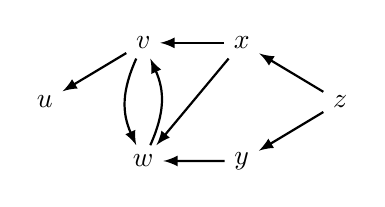
\begin{tikzpicture}[xscale=1.25, yscale=0.75]
      \node[vertex] (u) at (0, 0) {$u$};
      \node[vertex] (v) at (1, 1) {$v$};
      \node[vertex] (w) at (1, -1) {$w$};
      \node[vertex] (x) at (2, 1) {$x$};
      \node[vertex] (y) at (2, -1) {$y$};
      \node[vertex] (z) at (3, 0) {$z$};

      \draw[arrow] (v) to (u);
      \draw[arrow, bend right=15] (v) to (w);
      \draw[arrow, bend right=15] (w) to (v);
      \draw[arrow] (x) to (v);
      \draw[arrow] (x) to (w);
      \draw[arrow] (y) to (w);
      \draw[arrow] (z) to (x);
      \draw[arrow] (z) to (y);
    \end{tikzpicture}
    \caption{A conflict graph}\figlabel{ExamplePreCondensation}
  \end{subfigure}

  \begin{subfigure}[b]{0.3\textwidth}
    \centering
    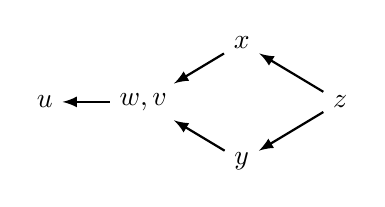
\begin{tikzpicture}[xscale=1.25, yscale=0.75]
      \node[vertex] (u) at (0, 0) {$u$};
      \node[vertex] (vw) at (1, 0) {$w,v$};
      \node[vertex] (x) at (2, 1) {$x$};
      \node[vertex] (y) at (2, -1) {$y$};
      \node[vertex] (z) at (3, 0) {$z$};

      \draw[arrow] (vw) to (u);
      \draw[arrow] (x) to (vw);
      \draw[arrow] (y) to (vw);
      \draw[arrow] (z) to (x);
      \draw[arrow] (z) to (y);
    \end{tikzpicture}
    \caption{The condensed conflict graph}\figlabel{ExampleCondensation}
  \end{subfigure}

  \caption{A conflict graph.}\figlabel{ExampleConflictGraph}
\end{floatingfigure}
}

The BPaxos protocols implement state machine replication by way of generalized consensus. We assume an asynchronous network model where processes can crash (but not act maliciously). More formally, we consider a set $\Cmd$ of commands and a symmetric binary relation $\conflict \subseteq \Cmd \times \Cmd$ called the conflict relation. We say two commands $x, y \in \Cmd$ conflict if $x \conflicts y$. A set of client processes propose commands to a set of state machine replicas (or replicas for short), and the replicas serially execute the commands with the following properties:

\vspace{3in}

The BPaxos protocols implement state machine replication by way of generalized consensus. We assume an asynchronous network model where processes can crash (but not act maliciously). More formally, we consider a set $\Cmd$ of commands and a symmetric binary relation $\conflict \subseteq \Cmd \times \Cmd$ called the conflict relation. We say two commands $x, y \in \Cmd$ conflict if $x \conflicts y$. A set of client processes propose commands to a set of state machine replicas (or replicas for short), and the replicas serially execute the commands with the following properties:





\paragraph{Approach 1.}
Every replica $r$ executes a sequence $\bar{x} = x_1, \ldots, x_n$. We say two
sequences $\bar{x}, \bar{y}$ are equivalent if there is a permutation between
them that preserves conflicts. We say two are compatible if there is an
extension of both that is equivalent.
  - stability: grows over time
  - consistency: any two are compatible


\paragraph{Approach 2.}
Every replica $r$ executes a sequence $\bar{x} = x_1, \ldots, x_n$. Assume
commands are distinct, because if not, we label them as distinct. If $x, x'$ conflict and $x$ precedes $x'$ in $r$'s sequence, then for every replica, if $x$ and $x'$ are executed, $x$ precedes $x'$.

Are these two equivalent????

\TODO{Think of a good section title.}
The BPaxos protocols implement state machine replication in an asynchronous model where processes can crash (but not act maliciously). More formally, we consider a set $\Cmd$ of commands and a symmetric binary relation $\conflict \subseteq \Cmd \times \Cmd$ called the conflict relation. We say two commands $x, y \in \Cmd$ conflict if $x \conflicts y$. A set of client processes propose commands to a set of state machine replicas (or replicas for short), and the replicas serially execute the commands with the following properties:

\TODO{Is this a good way to formalize the problem. EPaxos formalizes it a bit different. Generalized Paxos does it a bit different as well. I would just say we're implementing Generalized Paxos, but thinking of things in terms of state machine replication makes it a bit easier to understand why BPaxos' invariants are the way they are.}
\begin{itemize}
  \item Nontriviality: replicas only execute proposed commands.
  \item If any replica executes a pair of conflicting commands $x, y$ in some order (either $x$ before $y$ or $y$ before $x$), then every replica executes the commands in this order. Non-conflicting commands can be executed in any order.
\end{itemize}
\TODO[]{Is this actually the same as generalized consensus?}

This is equivalent to the replicas achieving generalized consensus on
Mazurkiewicz traces (or command histories), executing commands in trace order
(or topoligal order). We do not discuss liveness in this paper. We do not discuss linearizability.

\subsection{Overview}

inv 1: gadget chosen
inv 2: conflicts, then exists


- nontriviality : obvious
- stability: only add new things, so always prefix
- consistency :

\begin{itemize}
  \item Commands $x$, $y$, $z$
  \item Acceptors $a_1$, $a_2$, $a_3$
  \item Dependency Service Nodes $d_1$, $d_2$, $d_3$
  \item Bipartisan Paxos Nodes $b_1$, $b_2$, $b_3$
\end{itemize}



async network, f failures, crash stop, blah blah blah
state machine replication of commands
equivalent to generalized consensus on Mazurkiewicz traces / command histories
requirements taken from epaxos

ignore linearizability
ignore liveness

% Bipartisan Paxos
%   - problem set up
%     - describe the problem we are trying to solve: generalized consensus on
%       BPaxos on Mazurkiewicz traces.
%     - describe the correctness criteria: nontriviality, etc.
%     - describe the desirable features we'd also like: load balancing, low
%       commit latency.
%     - we'd also like to have it be simple.
%   - overview
%     - build graph
%     - execute one strongly connected component at a time
%     - two key invariants:
%        - gadgets chosen
%        - chosen conflicting commands have edge
%     - both are sufficent are to ensure the invariants above (short proof)
%     - second is actually necessary, first makes things much simpler
